%(BEGIN_QUESTION)
% Copyright 2006, Tony R. Kuphaldt, released under the Creative Commons Attribution License (v 1.0)
% This means you may do almost anything with this work of mine, so long as you give me proper credit

Beregn utgangsspenningen til denne brokoblingen ved følgende RTD-temperaturer (antar en 100 $\Omega$ RTD med europeisk alpha-verdi).

$$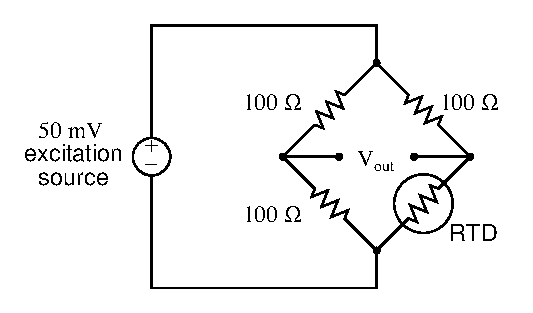
\includegraphics[width=15.5cm]{i00410x01.eps}$$

\begin{itemize}
\item{} $V_{out}$ = \underbar{\hskip 50pt} ved $T$ = 0$^{o}$ C
\vskip 5pt
\item{} $V_{out}$ = \underbar{\hskip 50pt} ved $T$ = 35$^{o}$ C
\vskip 5pt
\item{} $V_{out}$ = \underbar{\hskip 50pt} ved $T$ = $-15^{o}$ C
\end{itemize}

\vskip 20pt \vbox{\hrule \hbox{\strut \vrule{} {\bf Forslag til sokratisk diskusjon} \vrule} \hrule}

\begin{itemize}
\item{} Den lave spenningen (50 mV) fra «eksitasjonskilden» er ikke vilkårlig, men har en praktisk hensikt. Forklar hvorfor det er viktig at denne spenningskilden er liten i størrelse og ikke stor (for eksempel 5 volt eller 24 volt).
\item{} Anta at den eneste DC-kilden vi har tilgjengelig for å drive RTD-broen er en fast 24 V-kilde. Hvordan kan denne kilden brukes sammen med brokoblingen uten problemer med overbelastning av broen?
\item{} Velg en vilkårlig motstand i kretsen og tenk at den feiler (enten avbrudd eller kortslutning). Vil denne elektriske feilen få RTD-en til å se varmere ut enn den faktisk er, eller kaldere? Forklar svaret i detalj.
\end{itemize}

\underbar{file i00410}
%(END_QUESTION)





%(BEGIN_ANSWER)

\noindent
{\bf Delvis svar:}

\begin{itemize}
\item{} $V_{out}$ = 0.000 mV ved $T$ = 0$^{o}$ C
\vskip 5pt
\item{} $V_{out}$ = 1.578 mV ved $T$ = 35$^{o}$ C
\vskip 5pt
\item{} $V_{out}$ = -0.7433 mV ved $T$ = -15$^{o}$ C
\end{itemize}

%(END_ANSWER)





%(BEGIN_NOTES)

\begin{itemize}
\item{} $V_{out}$ = 0.000 mV ved $T$ = 0$^{o}$ C
\vskip 5pt
\item{} $V_{out}$ = 1.578 mV ved $T$ = 35$^{o}$ C  ($R_{RTD}$ = 113.475 $\Omega$)
\vskip 5pt
\item{} $V_{out}$ = $-0.7433$ mV ved $T$ = $-15^{o}$ C  ($R_{RTD}$ = 94.225 $\Omega$)
\end{itemize}


%INDEX% Measurement, temperature: RTD

%(END_NOTES)
